% Forløbig resultater
% Opsætning
% Fuel
% Afstand
% Fremtidige tests/arbejde
% Konklusion


\section{Evaluation}
\begin{frame}{Test Setup}



\begin{columns}
	\begin{column}{0.7\textwidth}
		\begin{itemize}
		\item SUMO- Simulation of Urban MObility\\
		\item Real world road network\\
		\item Real world Traffic light phases\\
		\item Real world OD matrix\\
		\end{itemize}
	\end{column}

	\begin{column}{0.3\textwidth}
		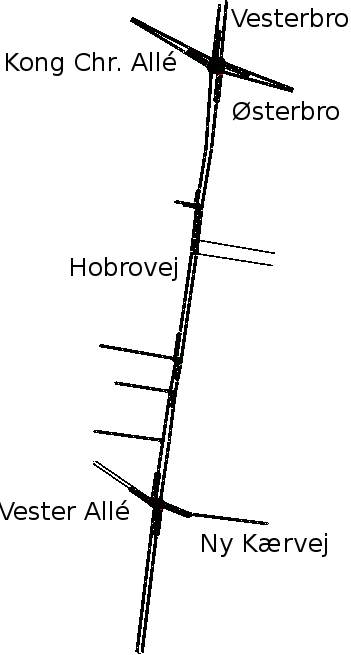
\includegraphics[width=0.8\textwidth]{images/Hobrovej.png}
	\end{column}
\end{columns}
\end{frame}

\begin{frame}{SUMO presentation}
\end{frame}

\begin{frame}{Fuelsaving}
	\begin{figure}
	\begin{tikzpicture}[scale=0.6]
	\begin{axis}[xlabel=Routes,xticklabel=\empty,ylabel=Fuel consumption,bar width=1pt,]
	\addplot[ybar, blue] table[x=Route,y=Fuel] {TestResults/0/avg.dat};
	\addplot[ybar, red] table[x=Route,y=Fuel] {TestResults/100/avg.dat};
	\draw[thick, red] (axis cs:0,138) -- (axis cs:109,138);
	\draw[thick, blue] (axis cs:0,162) -- (axis cs:109,162);
	\end{axis}
	\end{tikzpicture}
	\caption{Average fuel consumption with (red) and without \tech (blue)}\label{tik:fuel:avg}
	\end{figure}
\end{frame}

